% ======================= Pre-Amble =========================
      
%Format
\documentclass[11pt, oneside]{article}   	% use "amsart" instead of "article" for AMSLaTeX format 
                     						%imports package {article} and specify option(s) [11pt, oneside]
\usepackage{geometry}                		% See geometry.pdf to learn the layout options. There are lots. 
    \geometry{letterpaper}                   		% ... or a4paper or a5paper or ... 
    %\geometry{landscape}                		% Activate for rotated page geometry

\usepackage[parfill]{parskip}    		        % Activate to begin paragraphs with an empty line rather than an indent

    %Colours
    \usepackage{graphicx, subcaption}
    \usepackage[usenames, dvipsnames]{color}     % font colour:    \textcolor{<colour>}{text}
          									%highlight text:  \colorbox{<color>}{text}
    \usepackage{soul}						%highlight text: \hl{}     %only  yellow								
    									%list of colours: https://www.sharelatex.com/learn/Using_colours_in_LaTeX
    									
    %Bullets
    \usepackage{enumerate}     %specify type of enumeration: \being{enumerate}[<type of enumeration>]
    
    %Footnote Spacing
    \setlength{\footnotesep}{0.4cm}                  %specify spacing b/w footnotes
    \setlength{\skip\footins}{0.6cm}                    % space b/w footnotes and textbody


%Mattematics
    %American Mathematics Society packages
    \usepackage{amsmath}	   %math
    \usepackage{amssymb}       %symbols
    \usepackage{amsthm}          %theorems

    %QED
    \newcommand*{\QEDA}{\hfill\ensuremath{\blacksquare}}         %make qed filled square:    \QEDA
    \newcommand*{\QEDB}{\hfill\ensuremath{\square}}               %make qed empty square: \QEDB 
    
    \renewcommand\qedsymbol{\ensuremath{\blacksquare}}		%Proof environment


%Figures
\usepackage{caption}
\captionsetup[figure]{labelfont=bf}    %make figure labels boldface
\captionsetup[table]{labelfont=bf}     %make table labels boldface

\usepackage[hidelinks]{hyperref}                % Allows for clickable references

    %Tables
    \usepackage[none]{hyphenat}                    % Stops breaking-up words in a table (i.e. no hyphens)                                                             
    
    \usepackage{array}   
        \newcolumntype{x}[1]{>{\centering\let\newline\\\arraybackslash\hspace{0pt}}p{#1}}       %center fixed column width: x{<len>}                      
        \newcolumntype{$}{>{\global\let\currentrowstyle\relax}}                                                   % let us apply things (e.g. bold/italicize) to entire row            
        \newcolumntype{^}{>{\currentrowstyle}}
        \newcommand{\rowstyle}[1]{\gdef\currentrowstyle{#1} #1\ignorespaces}
    
    %Images
    \graphicspath{ {images/} }                          %directory that your images are located in within your current directory
    
    %Diagrams
    \usepackage[latin1]{inputenc}
    \usepackage{tikz}
    	\tikzset{line/.style={-latex'}}
        \usepackage{tkz-berge}
        \usetikzlibrary{shapes,arrows}
        \usetikzlibrary{patterns}			%Specify colours of stuff (e.g. vertices): 
        								%	-> set style: \tikzset{VertexStyle/.append style = {minimum size = 8pt, inner sep = 0pt}} 
								%	-> change individual vertices: \AddVertexColor{white}{1,2} 


%Bibliography
\usepackage[numbers,sort&compress]{natbib}   %for multiple references: sorts  (i.e. [1,2] NOT [2, 1] )
                                           				  %                                     compresses (i.e. [1-3] )
\usepackage[nottoc]{tocbibind}                            %add bibliography to table of contents


%Miscellaneous
\usepackage{dirtytalk}    %quotations: use \say  


%================== Header & Footer =========================
\usepackage{fancyhdr}
\usepackage{lastpage}      %ensures you can reference LastPage (i.e. Page 2 of 10)

\renewcommand{\headrulewidth}{0.4pt}		%Decorative Header line: thickness={0.4pt}
\renewcommand{\footrulewidth}{0.4pt}		%Decorative Footer line: thickness={0.4pt}

\setlength{\headheight}{13.6pt} 		%space b/w top of page & header
\setlength{\headsep}{0.3in}		%space b/w page header and body

%Make Header & Footer    
\pagestyle{fancy}
    \lhead{Stephanie Knill} 		% controls the left corner of the header
    \chead{} 					% controls the center of the header
    \rhead{} 					% controls the right corner of the header
    \lfoot{} 					% controls the left corner of the footer
    \cfoot{Page~\thepage\ of \pageref{LastPage}} 				% controls the center of the footer
    												%Page~\thepage\  if just want Page x
    \rfoot{}			 		% controls the right corner of the footer

% =============================== Document ===================================
\begin{document}

% Title Page
\title{MATH 442 --- Assignment 9 \\
\line(1,0){360} \\              %(slope x, y){length of line}
}
\author{
Stephanie Knill \\
54882113 \\
Due: March 17, 2016}

\date{}                   % Activate:  display a given date (e.g. {August 4} ) or no date (empty {} )
                                    %No activate: display current date
\maketitle

%\thispagestyle{empty}                   %Remove header from this (first) page. Change empty -> plain to keep numbering
%								-> Doesn't matter in this case (b/c title page)
%\cleardoublepage


% ================= Questions ================

\section*{Question 49}

From our lecture timetable, we can construct a graph $G$ (Figure \ref{q1}) where each vertex represents a lecture period and two lecture periods are adjacent if they must not coincide.

\begin{figure}[h]
	\centering
        \begin{tikzpicture}[scale=0.75,transform shape]
		
		%\GraphInit[vstyle=Classic]					%Make vertice labels outside it
		%\SetVertexNoLabel							%No vertice labels
		\tikzset{VertexStyle/.append style = {circle}}		%Set vertex style
			\Vertices[unit=4]{circle}{c,b,a,g,f,e,d}
			%\AddVertexColor{white}{1,2} 					%Change individual vertex type
    
		\path [thick] (a) edge (b);			%arrows: [line];     label: {$label}$
    		\path [thick] (b) edge (c);	
    		\path [thick] (c) edge (d);	
    		\path [thick] (d) edge (e);	
    		\path [thick] (e) edge (f);
    		\path [thick] (f) edge (g);
    		\path [thick] (g) edge (a);
		
		\path [thick] (a) edge (c);
		\path [thick] (a) edge (d);
		\path [thick] (b) edge (d);
		\path [thick] (b) edge (e);
		\path [thick] (b) edge (g);
		\path [thick] (c) edge (f);
		
    	\end{tikzpicture}  
        \caption{Graph $G$ where each vertex represents a lecture period and two lecture periods are adjacent if they must not coincide.}
        \label{q1}
 \end{figure}

To determine the minimum number of lecture periods needed to timetable all 7 lectures, we need to calculate the chromatic index $\chi(G)$---the minimum number of colours needed to colour the vertices of $G$. Using Brooke's Theorem, the largest degree $\Delta =5$, so $G$ is 5-colourable. Now that we have estabilished an upper bound on $\chi(G)$, let us see if we can do better. Using the 4-colour Theorem, we know that if $G$ is planar, then $G$ is 4-colourable. Using Glasgow's Algorithm (Figure \ref{glasgow})

\begin{figure}[h]
	\centering
        \begin{tikzpicture}[scale=0.75,transform shape]
		
		%\GraphInit[vstyle=Classic]					%Make vertice labels outside it
		%\SetVertexNoLabel							%No vertice labels
		\tikzset{VertexStyle/.append style = {circle}}		%Set vertex style
			%\AddVertexColor{white}{1,2} 					%Change individual vertex type
			\Vertex [x=0,y=0]{cf}
			\Vertex [x=0,y=2]{ad}
			\Vertex [x=0,y=4]{ac}
			\Vertex [x=4,y=4]{bd}
			\Vertex [x=4,y=2]{be}
			\Vertex [x=4,y=0]{bg}
    
		\path [thick] (cf) edge (ad);			%arrows: [line];     label: {$label}$
		\path [thick] (ac) edge (bd);
		\path [thick] (ac) edge (be);
		\path [thick] (ac) edge (bg);
		\path [thick] (ad) edge (be);
		\path [thick] (ad) edge (bg);
		\path [thick] (cf) edge (be);
		
    	\end{tikzpicture}  
        \caption{Graph $H$ generated from $G$ using Glasgow's Algorithm.}
        \label{glasgow}
 \end{figure}
 We see there exists a cycle of length 3 $ad \to be \to cf \to ad$, thus $H$ is not bipartite and $G$ is not planar. Since we cannot do better, $G$ is 5-chromatic and we need 5 lecture periods.

\section*{Question 50}

There are five teams playing in a tournament, each playing the other four teams once and with two pitches available. Let us express our tournament as the connected graph $K_5$ of number of vertices $n=5$. To determine the number of periods needed to schedule all the matches, we need to find the minimum number of colours required to colour the edges, or $\chi '(K_5)$. Since $n$ is odd, we have that $\chi '(K_5) = n = 5$. So we need 5 periods if we have an unlimited number of pitches to play on. However, having an unlimited or 2 pitches is the same as a team cannot play 2 matches simultaneously. This means we can have at most 2 games played in a single period, thus we need 5 periods.



\section*{Question 51}

A simple connected graph $T$ is a tree if and only if $v=e+1$.

\begin{proof}
$\Rightarrow$ Assume the simply connected graph $T$ is a tree. Since it is planar, we can apply Euler's Theorem to it
$$v - e + f = 2$$
Here, no cycles exist, so we only have the infinite face and $f=1$. Substituting this in gives us
\begin{align*}
	v - e + 1 & = 2 \\
	v & = e+ 1
\end{align*}
$\Leftarrow$ Assume to the contrary that the graph $T$ has $v=e+1$ and it is not a tree. Thus we must have a cycle in $T$. To connect our $v$ vertices into a cycle, we need at least $v$ edges. However, we only have $e=v-1$ edges, thereby giving us the necessary contradiction.
\end{proof}


\section*{Question 52}

Prove that a simple connected graph $T$ is a tree if and only if adding an edge between two existing vertices of $T$ creates exactly one cycle.
\begin{proof}
$\Rightarrow$ Assume that $T$ is a tree. Then there exists a path between any 2 vertices $v_i$ and $v_j$. If we join vertex $v_i$ and $v_j$ we will form a cycle of the form $v_i \to \cdots \to v_j \to v_i$. By Lemma, this is the only cycle formed. 

\emph{Lemma} Assume that adding an edge $e$ in a tree creates more than 1 cycle. Adding $e$ between $v_i$ and $v_j$ forms at least 2 cycles (Figure \ref{q52})

\begin{figure}[h]
	\centering
        \begin{tikzpicture}[scale=0.75,transform shape]
		
		%\GraphInit[vstyle=Classic]					%Make vertice labels outside it
		%\SetVertexNoLabel							%No vertice labels
		\tikzset{VertexStyle/.append style = {circle}}		%Set vertex style
			%\AddVertexColor{white}{1,2} 					%Change individual vertex type
			\Vertex [x=0,y=0, L=$v_1$]{1}
			\Vertex [x=3,y=0, L=$v_2$]{2}
    
		\path [solid] (1) edge [out=90,in=90, bend angle=100] (2);			%arrows: [line];     label: {$label}$
		\path [solid] (2) edge [out=-90,in=-90, bend angle=100] (1);	
		\path [dashed] (1) edge (2);
		
    	\end{tikzpicture}  
        \caption{Cycles formed from adding edge $e$ dashed between vertices $v_i$ and $v_j$.}
        \label{q52}
 \end{figure}
 However, this implies that a cycle already existed in $T$ of the form $v_i \to \cdots \to v_j \to \cdots \to v_i$, which contradicts the definition of a tree.


$\Leftarrow$ Assume that adding an edge $e$ between any two existing vertices of $T$ creates exactly one cycle. Then we have 3 cases. In the first case, we added $e$ to the same vertex, forming a loop. This cycle would result in any graph. Similarly in the case where we add $e$ to any two adjacent vertices, we form multiple edges, thus again resulting a cycle. Again, this can occur in any graph.

Let us examine the final case where we add an edge $e$ between any two non-adjacent vertices $v_i$ and $v_j$. To form a cycle, then there must exist exactly 1 path between $v_i$ and $v_j$. Otherwise, if there were none, we would not form a cycle. If there were more than 1 path, a cycle would have already existed involving $v_i$ and $v_j$ and we would form more than 1 cycle. By definition then $T$ must be a tree.
\end{proof}
\section*{Question 53}

Prove that a forest with $n$ vertices and $k<n$ has $n-k$ connected components. 
\begin{proof}

Since a forest is a union of trees $T_1, T_2, \ldots , T_m$, where each tree $T_i$ has number of vertices $n_i = k_i +1$ by Lemma. So we have that $n_i-k_i = 1$. Let $n=n_1+ \ldots + n_m$ and  $k = k_1 + \ldots k_m$, where $m$ is the number of components. Then
\begin{align*}
	m & = 1 + 1 + \ldots + 1 \\
	& = (n_1-k_1) + (n_2 - k_2) + \ldots + (n_m - k_m) \\
	& = n-k
\end{align*}
\end{proof}

\emph{Lemma: Any tree with $n$ vertices contains precisely $n-1$ edges.}

We will proceed by induction over the number of vertices $n$.

\textbf{Base Case:} When $n=1$, we have the null graph $N_1$ of 0 edges.

\textbf{Induction Step:} Let $k \in \mathbb{N}$ be given and suppose the statement is true for $n=k$ vertices. Let $G$ denote the tree of $k$ vertices that has $k-1$ edges by the induction assumption. Let us add a vertex $v$ to $G$. Since the resulting graph must be connected, we have two cases:

\emph{Case 1:} Join $v$ to $G$ with 1 edge. Here we have $k+1$ vertices and $k$ edges, so we are done.

\emph{Case 2:} Join $v$ to $G$ with at least 2 edges. Since there exists a path between any two vertices $v_i$ and $v_j$ in $G$, if we join vertex $v$ to both $v_i$ and $v_j$ we will form a cycle of the form
$$v\rightarrow v_i\rightarrow \cdots \rightarrow v_j \rightarrow v$$
which is not allowed.

Thus, the statement holds for $n=k+1$, and the proof of the induction step is complete.

\textbf{Conclusion:} By the principle of induction the statement is true for all $n$.



\section*{Question 54}

Let $T$ be a tree with no vertices of degree 2. Prove that $T$ has more leaves than non-leaf vertices.

\begin{proof}
We will proceed by induction over the number of vertices $n$.

\textbf{Base Case:} When $n=2$, we have 2 leaves and 0 non-leaf vertices.

\textbf{Induction Step:} Assume true for $2 < n \leq k$ vertices. Let $G$ be such a graph of $k$ vertices. Let us add a vertex $v$ to our graph to form $G'$ of $n=k+1$ vertices. Since no vertex can be of degree 2, then we cannot add $v$ to a leaf. Adding $v$ to a non-leaf means we have the same number of non leafs and an additional leaf. Since be the induction assumption we have more leaves than non-leaves in $G$, then $G'$ also has more leaves.

\textbf{Conclusion:} By the principle of induction the statement is true for all $n$.
\end{proof}


\end{document} 